\documentclass[11pt,reqno,final]{amsart}

\pdfcompresslevel=0
\pdfobjcompresslevel=0

\usepackage[dvipsnames]{xcolor}% adds colors
\usepackage{amsmath, amsthm}% {amsfonts, amssymb}

% New Characters
\usepackage[latin1]{inputenc}%
\usepackage[T1]{fontenc}

\usepackage{MnSymbol}

\usepackage[theoremfont,largesc]{newpxtext} % different text,math font
\usepackage{newpxmath}

\usepackage[normalem]{ulem}% underlining
\usepackage{bbm}% more bb





% Page Typesetting
\usepackage[final]{microtype}
\usepackage{relsize}
\usepackage[margin=1in]{geometry}
\usepackage{framed}
\usepackage{tikz}

\usepackage[inline,shortlabels]{enumitem}% % can use \begin{enumerate*} for inparaenum

\usepackage{hyperref}
\hypersetup{
  final,
  pdftitle={Math 135 - Modeling with Functions},
  pdfauthor={Bonventre}, 
  linktoc=page,
  pagebackref,
  colorlinks=true,
  citecolor=PineGreen,
  linkcolor=PineGreen,
  linkbordercolor=PineGreen,
}


% Internal References

\numberwithin{equation}{section} 
\numberwithin{figure}{section}

\usepackage[nameinlink,capitalise,noabbrev]{cleveref}

\crefname{equation}{}{} % get \cref to behave as \eqref

% \theoremstyle{plain} % bold name, italic text
\newtheorem{theorem}[equation]{Theorem}%
\newtheorem*{theorem*}{Theorem}%
\newtheorem{lemma}[equation]{Lemma}%
\newtheorem{proposition}[equation]{Proposition}%
\newtheorem{corollary}[equation]{Corollary}%
\newtheorem{conjecture}[equation]{Conjecture}%
\newtheorem*{conjecture*}{Conjecture}%
\newtheorem{claim}[equation]{Claim}%
\newtheorem{question}{Question}

\theoremstyle{definition} % bold name, plain text
\newtheorem{definition}[equation]{Definition}%
\newtheorem*{definition*}{Definition}%
\newtheorem{example}[equation]{Example}%
\newtheorem*{example*}{Example}%
\newtheorem{remark}[equation]{Remark}%
\newtheorem{notation}[equation]{Notation}%
\newtheorem{convention}[equation]{Convention}%
\newtheorem{assumption}[equation]{Assumption}%
\newtheorem{exercise}[question]{Exercise}

% ---------- macros

\newcommand{\set}[1]{\left\{#1\right\}}%
\newcommand{\sets}[2]{\left\{ #1 \;|\; #2\right\}}%
\newcommand{\longto}{\longrightarrow}%
\newcommand{\into}{\hookrightarrow}%
\newcommand{\onto}{\twoheadrightarrow}%

\usepackage{harpoon}
\newcommand{\vect}[1]{\text{\overrightharp{\ensuremath{#1}}}}


\newcommand{\del}{\partial}%

\newcommand{\ki}{\chi}
\newcommand{\ksi}{\xi}
\newcommand{\Ksi}{\Xi}


% %%%%%%%%%%%%%%%%%%%%%%%%%%%%%%%%%%%%%%%%%%%%%%%%%%%%%%%%%%%%%%%%%%%%%%%%%%%%%%%%%%%%%%%%%%%%%%%%%%%%

\begin{document}

%\maketitle
\begin{center}
        \textbf{\Large Math 135, Calculus 1, Fall 2020}\\[10pt]
        {\large 09-07: Modeling with Functions (Sections 1.1, 1.2, 1.6)}
\end{center}

\thispagestyle{empty}

\renewcommand{\thesection}{\Alph{section}}

\section{Meet your classmates}

Discuss what you have in common with your classmates, and what distinguishes you:
\begin{question}
        Create a 3-circle Venn Diagram, one for each member of your breakout room.
        Try to find several items to fit into each of the 7 sections.
        Examples could be: what year are you? where are you living? what is your favorite book? what major are you? where do you like to eat around town? where is somewhere you would like to travel? what helps you relax during quarantine?
\end{question}

\section{Linear Functions}

\begin{framed}
        A \textbf{linear function} is a function of the form $f(x) = mx + b$, where $m$ and $b$ are real numbers.
        It's graph is a line.
        The constant $m$ is the \textbf{slope} of the line.:
        for any two points $(x_1, y_1)$ and $(x_2, y_2)$ on the line, the slope is given by
        \[
                m = \dfrac{\mbox{change in $y$}}{\mbox{change in $x$}} = \dfrac{\Delta y}{\Delta x} = \dfrac{y_2 - y_1}{x_2 - x_1}
        \]
        The slope of a line determines the rate that $y$ changes as a function of $x$.
        
        The constant $b$ is the \textbf{$y$-intercept}, the value $f(0)$.
\end{framed}

\subsection*{Point-slope form}
If we know the slope of a line is $m$, and we have a point $(x_0,y_0)$ on the line,
then the equation for the line is given by
\[
        y - y_0 = m(x-x_0).
\]

\subsection*{Properties:}
\begin{itemize}
\item A line is \textbf{increasing} if $m > 0$, and \textbf{decreasing} if $m < 0$
\item A line with slope $m = 0$ is horizontal, and is a constant function.
\item Two lines are \textbf{parallel} if their slopes are equal, and \textbf{perpendicular} if the product of their slopes is $-1$.
\end{itemize}


\begin{exercise}
        \label{computerex}
        A computer is purchased for \$2816, and depreciates at a constant rate to \$0 in 8 years.
        \begin{enumerate}[(a)]
        \item  Find a formula for the value, $V$, of the computer after $t$ years have passed, and
                use this formula to give the value of the computer after 5 years.
                \vfill
                \vfill
        \item Under this model, what is the value of the computer after 9 years? What does this mean?
                \vfill
        \item What percent of the \textbf{initial} values does the computer lose per year?
                \vfill
        \end{enumerate}
\end{exercise}

\newpage

\section{Exponential Functions}

\begin{framed}
        An \textbf{exponential function} if a function of a form $f(x) = b^x$ for some positive constant $b > 0$.
        These functions model quantities that grow or decay based on how much of that quantity is currently present.
\end{framed}

\subsection*{Warning:} The variable in an exponential function is an \textbf{exponent}.
There is a huge different between
$x^2$ (the Squaring Function) and $2^x$ (the Doubling Function).\\

We'll work with these in more detail later, but let's see some first properties:

\subsection*{Properties:}
\begin{itemize}
\item Exponential functions grow very, very fast.
\item The domain of any exponential function is all real numbers.
\item The \textbf{base} of an exponential function is the constant $b > 0$.
\item If $b > 1$, the function is always increasing and we have exponential \textbf{growth};
        if $b < 1$, the function is always decreasing and we have exponential \textbf{decay}.
        \begin{figure}[ht]
                \begin{minipage}{0.4\linewidth}
                        \begin{center}
                                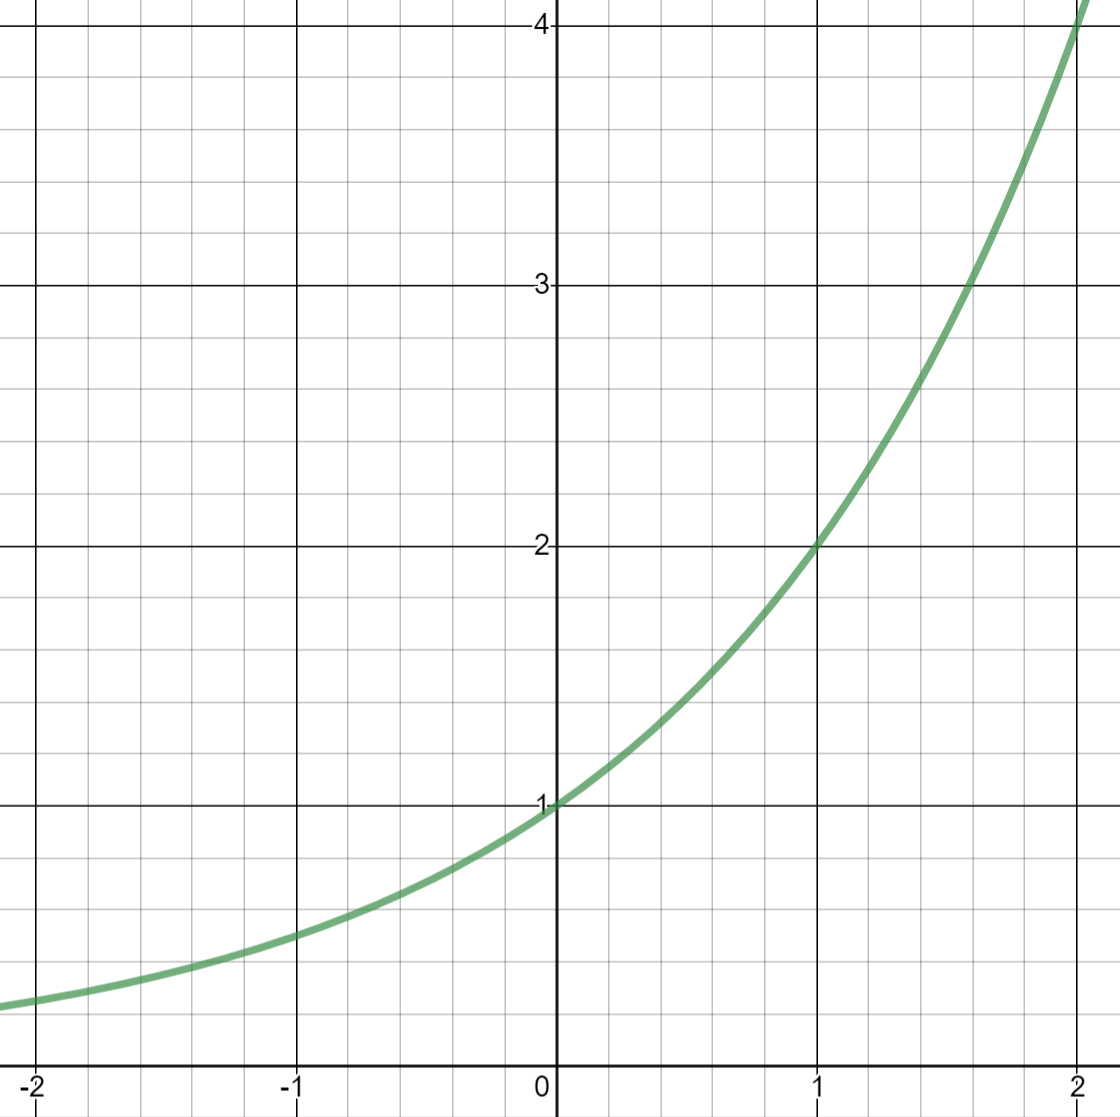
\includegraphics[width=1.5in]{09-07P_exp1.png}
                        \end{center}
                \end{minipage}
                \begin{minipage}{0.4\linewidth}
                        \begin{center}
                                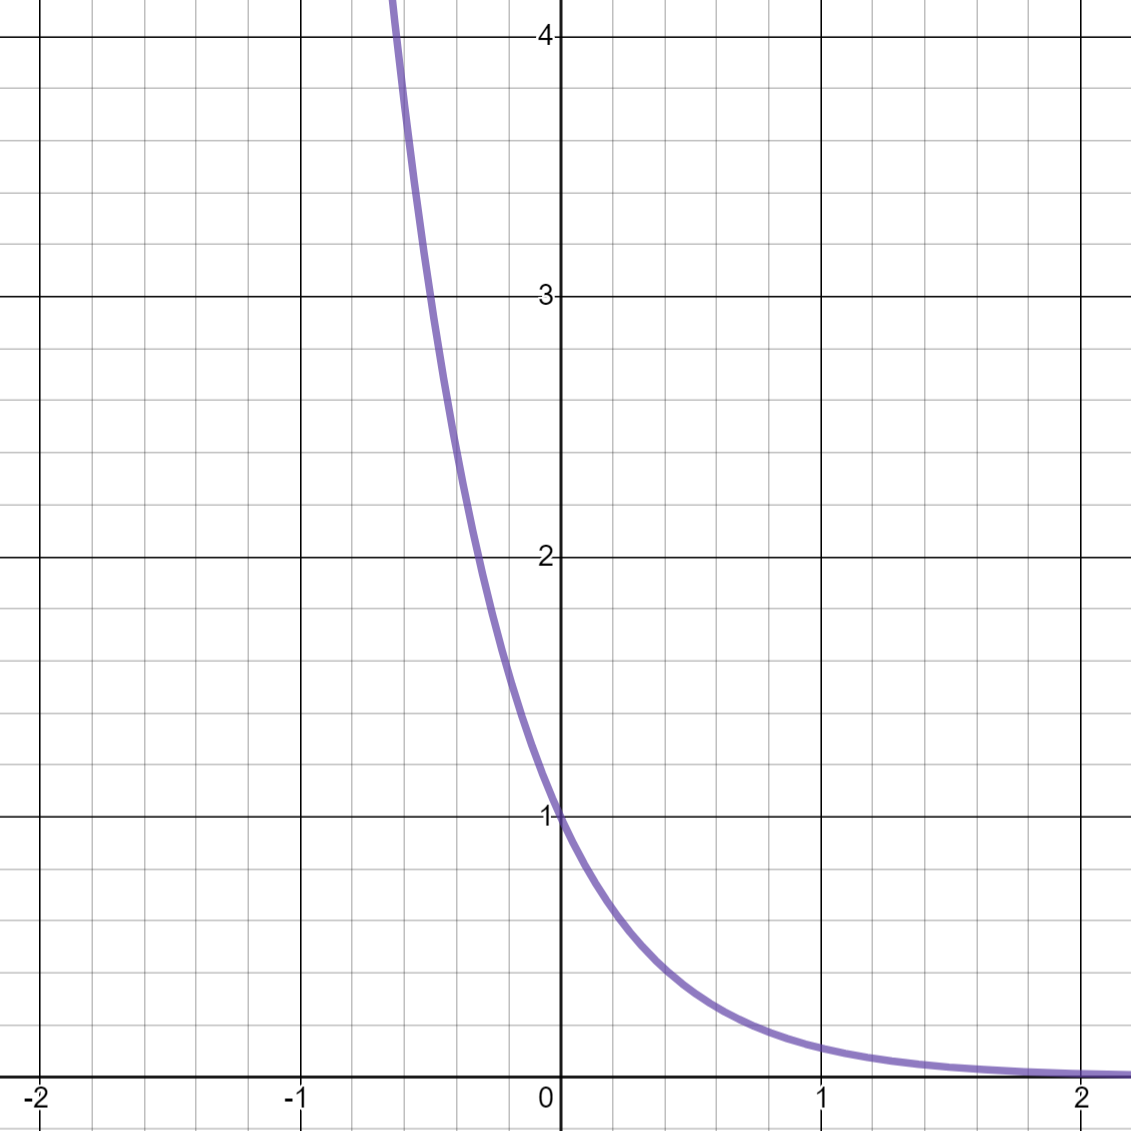
\includegraphics[width=1.5in]{09-07P_exp2.png}
                        \end{center}
                \end{minipage}
                \caption{$f(x) = 2^x$ (growth) and $g(x) = 3^{-2x}$ (decay)}
        \end{figure}
\item If the quantity $Q$ changes by $p$ percent every $t$ units of time, then the quantity is modeled by
        \[
                Q(t) = Q_0 \cdot p^{x/t}
        \]
        where $Q_0$ is the initial quantity.
\end{itemize}

\begin{example*}
        Over the course of 60 minutes, a colony of E. coli bacteria will grow by 118 percent.
        If we began with 100 bacteria, then the size of the colony after $x$ minutes is modeled by
        \[
                Q(t) = 100 \cdot (2.18)^{x/60}.
        \]
\end{example*}

\begin{exercise}
        Let's consider a different model for depreciation of the comptuer from \cref{computerex},
        one which models items which depreciate faster early in their life:
        We double the depreciation rate (from \cref{computerex} Part(c)), and each year the object loses that percentage of its \textbf{current} value.
        \begin{enumerate}[(a)]
        \item Find a formula that fits this model, and
                use this formula to give the value of the computer after 5 years.
                \vfill
                \vfill
        \item What are some purchases whose values might be better modeled by the second version?
                \vfill
        \end{enumerate}        
\end{exercise}


\newpage




\section{Modeling with Functions}

\begin{exercise}
        A light-rail system carries 80000 passengers per day at a fare of \$2.25 per ride.
        For each 5-cent increase in fare, surveys predict ridership will drop by 250 passengers.
        Call $x$ the number of 5-cent increases.
        \begin{enumerate}[(a)]
        \item Write a formula for the number of riders as a function of $x$.
                \vfill
        \item Write a formula for the fare per ride as a function of $x$.
                \vfill
        \item Write a function that gives the revenue as a function of $x$.
                \vfill
        \item Graph the revenue function using \href{https://www.desmos.com/}{Desmos} or a graphing calculator.
                \begin{center}
                        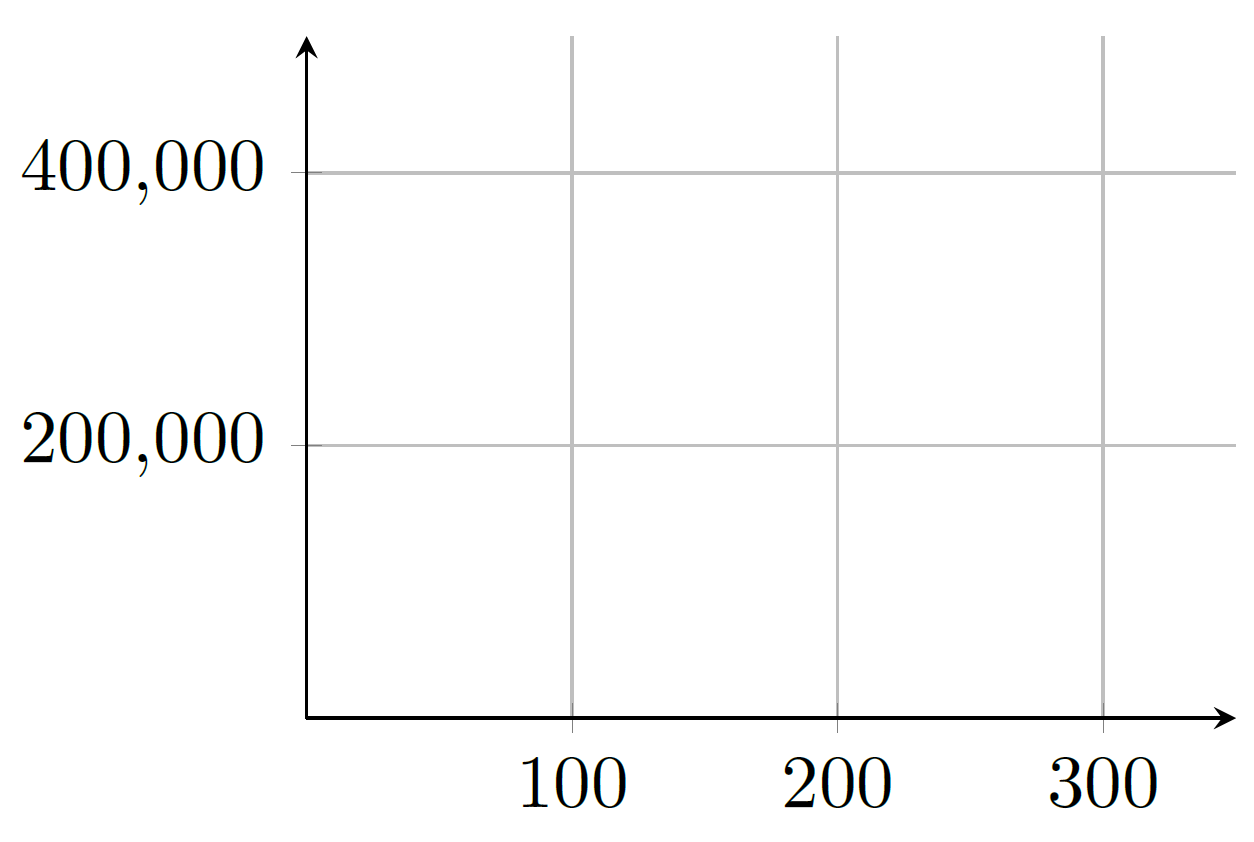
\includegraphics[width=3in]{09-07P_graph1.png}
                \end{center}
        \item From the graph, estimate the maximum revenue and the fare that will produce this revenue.
                \vfill
        \end{enumerate}
\end{exercise}

\newpage

\begin{exercise}
        In 1969, the world record time for the mile was 4:36.8, held by Maria Gommers.
        In 1980, the world record was held by Mary Slaney, with a time of 4:21.7.
        \begin{enumerate}[(a)]
        \item Find a linear model that fits this data, and use it to predict the world record time in 1996 and 2050.
                \vfill
                \vfill
        \item What is the slope of your linear model? What does it represent (include units)?
                \vfill
        \item If $t$ represents the year, what is the $t$-intercept of your linear model?
                Including units, what does it represent?
                Comment on the validity of the model.
                \vfill
        \item Using the same data, now construct an exponential model
                (Hint: $p$ should equal a certain ratio of times, and $t$ the number of years passed).
                Use this model to predict the world record time in 1996 and 2050.
                \vfill
                \vfill
        \item What is the $t$-intercept of your exponential model? What is the end behavior, and what does it represent?
                \vfill
        \item In 1996, the world record was set by Svetlana Masterkova, in a time of 4:12.56.
                How well did each model predict this?
                \vfill
        \end{enumerate}
\end{exercise}



\end{document}